\documentclass{article}
\usepackage{amsmath}
\usepackage{amssymb}
\usepackage[pdftex]{graphicx}
\usepackage[]{mcode}

\pdfpagewidth 8.5in
\pdfpageheight 11in
\topmargin -1in
\headheight 0in
\headsep 0in
\textheight 8.5in
\textwidth 6.5in
\oddsidemargin 0in
\evensidemargin 0in
\headheight 50pt
\headsep 0in
\footskip .75in

\title{STA 601 - Homework 6}
\author{Kedar Prabhudesai}
\date{September 19, 2013}

\begin{document}
\maketitle

\begin{enumerate}
\item \underline{Data:}\\
$y_i \sim \mathcal{N}_2(\mu,\Sigma)$, $i = 1,2,\ldots,100.$\\
$\mu = \left[\begin{matrix}0\\0\end{matrix}\right]$, $\Sigma = \left[\begin{matrix}1 & \rho\\\rho & 1\end{matrix}\right]$, $\rho=0.8.$\\

\item \underline{Maximum Likelihood Estimates:}\\
$\mu_{MLE} = \left[\begin{matrix}0.0715\\0.0969\end{matrix}\right]$\\
$\Sigma_{MLE} = \left[\begin{matrix}1.0789 & 0.9091\\0.9091 & 1.1541\end{matrix}\right]$\\

\begin{left}
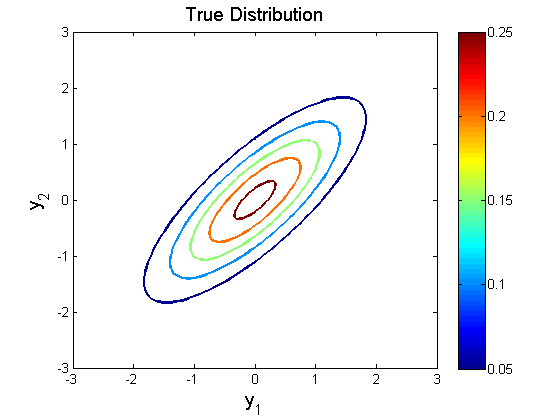
\includegraphics[scale=0.5]{TrueDist.png}
\end{left}
\begin{right}
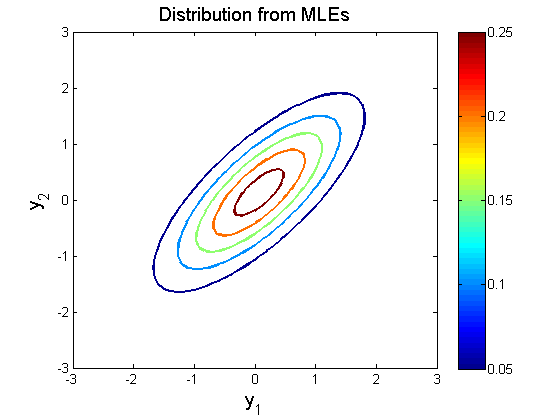
\includegraphics[scale=0.5]{MLEDist.png}\\
\end{right}
\begin{center}
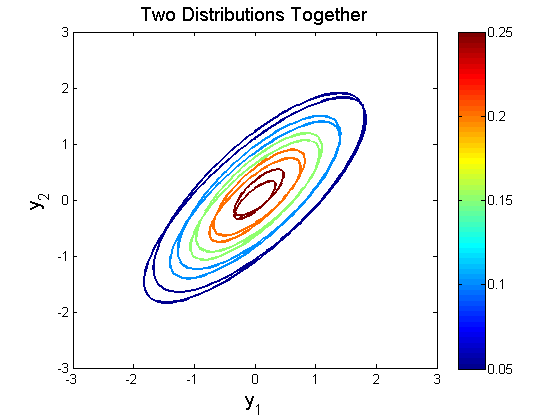
\includegraphics[scale=0.5]{TrueAndMLE.png}\\
\end{center}

\pagebreak

\item \underline{Gibbs Sampling:}\\
I used the following priors:\\
$\mu \sim \mathcal{N}_2\left[\left(\begin{matrix}0.2\\0.2\end{matrix}\right),\left(\begin{matrix}1.25 & 0.6\\0.6 & 1.25\end{matrix}\right)\right].$ 
$\Sigma \sim$ Inverse-Wishart$\left[4,\left(\begin{matrix}1.2 & 0.4\\0.4 & 1.2\end{matrix}\right)^{-1}\right].$\\
Also, I used 10,000 samples and burn-in of 1000.

\item \underline{Estimates from Posterior:}\\
$\mu_{posterior} = \left[\begin{matrix}0.0735\\0.0994\end{matrix}\right]$\\
$\Sigma_{posterior} = \left[\begin{matrix}1.0791 & 0.9031\\0.9031 & 1.1551\end{matrix}\right]$\\$

\item \underline{Comparison:}\\
If we compare the Bayes estimates and MLEs, they are very close to the true values of $(\mu,\Sigma)$

\end{enumerate}

\pagebreak
\noindent {\Large\underline{\textbf{Appendix:}}}\\
\lstinputlisting{C:/Users/ksp6/Documents/Classes/2013-Fall/STA601-BayesAndModStats/homeworks/hw6/hw6.m}

\end{document}